\documentclass[11pt]{article}
\usepackage[letterpaper]{geometry}
\usepackage{listings}
\usepackage{color}
\usepackage{graphicx}
\definecolor{dkgreen}{rgb}{0,0.6,0}
\definecolor{gray}{rgb}{0.5,0.5,0.5}
\definecolor{mauve}{rgb}{0.58,0,0.82}

\lstset{frame=tb,
	language=C,
	aboveskip=3mm,
	belowskip=3mm,
	showstringspaces=false,
	columns=flexible,
	basicstyle={\small\ttfamily},
	numbers=none,
	numberstyle=\tiny\color{gray},
	keywordstyle=\color{blue},
	commentstyle=\color{dkgreen},
	stringstyle=\color{mauve},
	breaklines=true,
	breakatwhitespace=true,
	tabsize=3
}


\title{\textbf{Tarea: Calculadora con procesos}}
\author{Diego Ruiz Mora | 2202000335}
\date{9-Septiembre-2023}

\begin{document}
		
	\maketitle
	\section{Creación de procesos para cada operación}
	Para iniciar, será necesario crear los procesos que nos ayudarán a realizar las operaciones correspondientes de suma, resta, multiplicación y división. En los cuales el código es bastante sencillo, como podemos apreciar en los siguientes imágenes:
	
	\begin{figure}[h!]
		\centering
		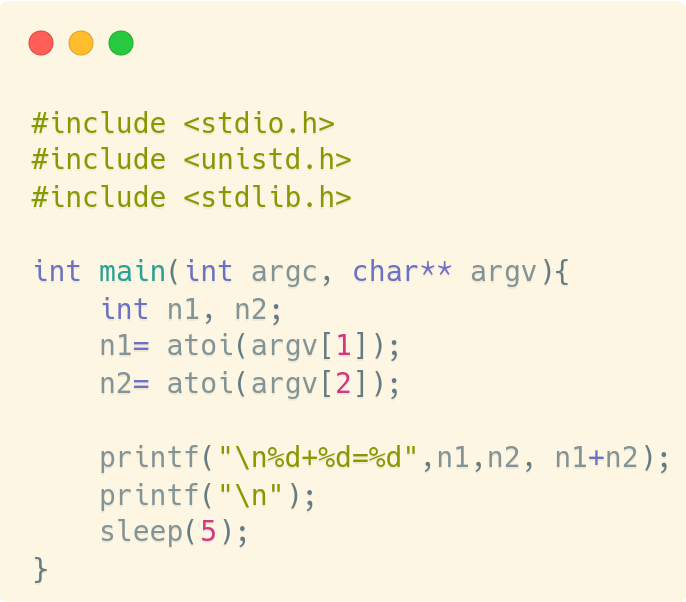
\includegraphics[width=0.5\linewidth]{suma.png}
		\caption{Código de suma.c}
		\label{fig:suma}
	\end{figure}
	
	Podemos notar de manera clara que en el código recibimos los parámetros, que en este caso tenemos el primero de ellos se refiere a la longitud del vector, que es el segundo parámetro que pasamos al 'main'. Este vector es de cadenas que termina con un '\textbf{NULL}, y al inicio tiene el comando con él que se invoca el programa, que en este caso sería \textbf{./suma}, en el medio tenemos algunos otros argumentos que se utilizarán en la ejecución de las instrucciones. 
	\\\\ 
	Esto se ve posteriormente en el código cuando de la tercera y cuarta posición del vector de argumentos obtenemos los números que vamos a sumar. Seguido, al efectuar la operación directamente lo imprimimos. Lo mismo sucederá en los siguientes casos, ya que las 4 primeras operaciones son sencillas de implementar. 
	\begin{figure}[h!]
		\centering
		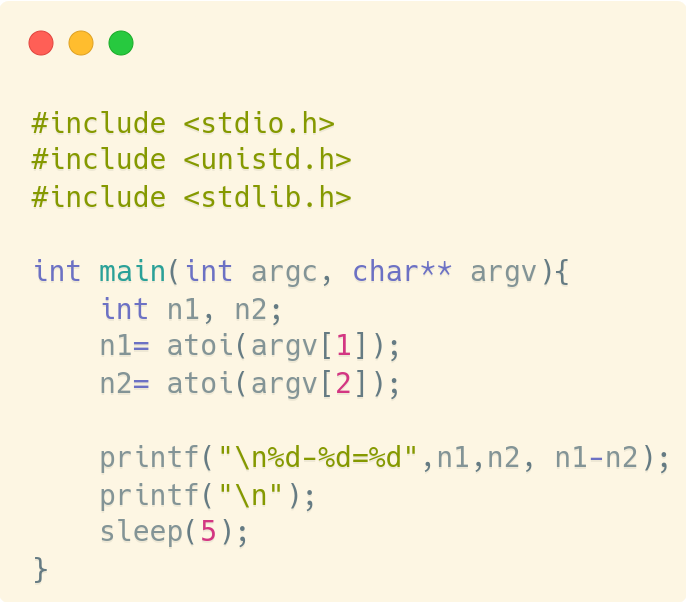
\includegraphics[width=0.5\linewidth]{resta.png}
		\caption{Código de resta.c}
		\label{fig:resta}
	\end{figure}
	\begin{figure}[h!]
		\centering
		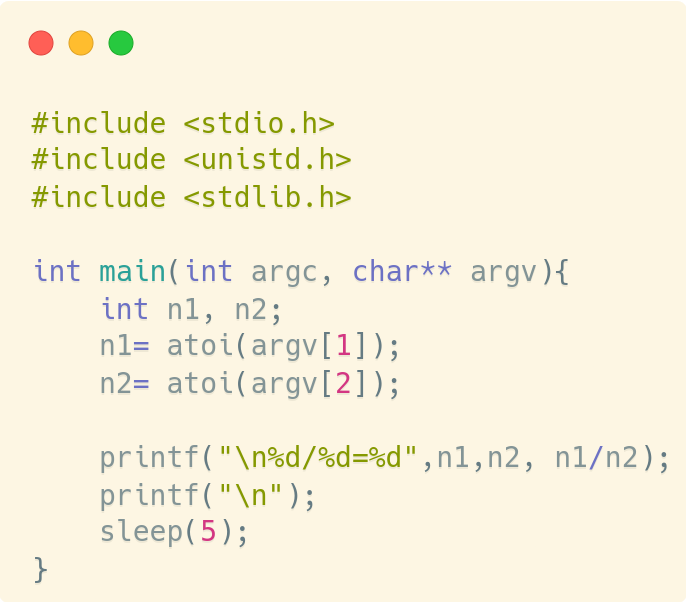
\includegraphics[width=0.5\linewidth]{division.png}
		\caption{Código de división.c}
		\label{fig:divsion}
	\end{figure}
	\begin{figure}[h!]
		\centering
		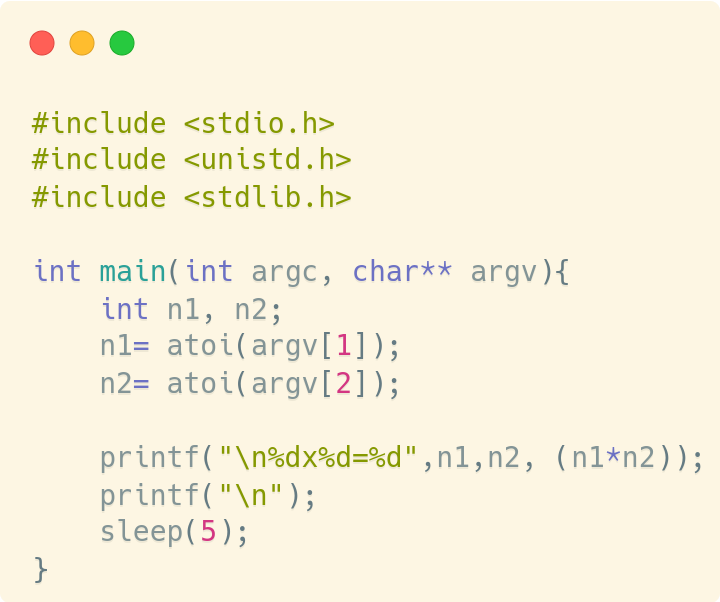
\includegraphics[width=0.5\linewidth]{multiplicacion.png}
		\caption{Código de multiplicación.c}
		\label{fig:multiplicacion}
	\end{figure}
	
\end{document}